\section{Associação de resistores: mista}

\frame{
	\frametitle{Definição}
	\begin{block}{Associação mista}
		Na associação de resistores mista, os resistores são ligados em série e em paralelo. Para calculá-la, primeiro encontramos o valor correspondente à associação em paralelo e de seguida somamos aos resistores em série.
	\end{block}

	\bigskip
	\centering
	\setmyunit{2cm}
	
	\begin{circuitikz}
		\draw (0,0) to[short,o-*] ++(0.5,0) -- ++(0,0.5)
		to[R,l=$ R_1 $] ++(1,0) -- ++(0,-1)
		to[R,l=$ R_2 $] ++(-1,0) -- ++(0,0.5)
		(1.5,0) to[R,l=$ R_3 $,*-o] ++(1,0);
	\end{circuitikz}
%	\centerline{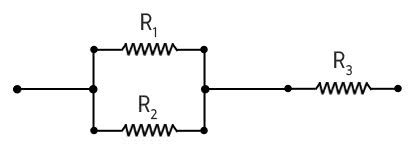
\includegraphics[width=0.8\linewidth]{Figuras/Ch15/mista.jpg}}
}

\frame{
	\frametitle{Associação mista}
	\begin{block}{Exemplo \#01}
		(PUC/RJ - 2018) Um circuito tem $3$ resistores idênticos, dois deles colocados em paralelo entre si, e ligados em série com o terceiro resistor e com uma fonte de \SI{12}{\volt}. A corrente que passa pela fonte é de \SI{5.0}{\milli\ampere}. Qual é a resistência de cada resistor, em $\si{\kilo\ohm}$?
	\end{block}
}

\frame{
	\frametitle{Associação mista}
	\begin{block}{Exemplo \#02}
		Determine a resistência equivalente entre os terminais $A$ e $B$ da seguinte associação de resistores:
	\end{block}

	\bigskip
	\centering
	\setmyunit{2cm}
	
	\begin{circuitikz}
		\draw (0,0) node[left] {$ A $} to[R=4<\ohm>,o-*] ++(1.5,0) -- ++(0.5,0.5)
		to[R=4<\ohm>] ++(1,0) -- ++(0.5,-0.5)
		(1.5,0) to[R=4<\ohm>] ++(2,0)
		(1.5,0) -- ++(0.5,-0.5) to[R=4<\ohm>] ++(1,0) -- ++(0.5,0.5) to[R=4<\ohm>,*-o] node[right] {$ B $} ++(1.5,0);
	\end{circuitikz}

%	\centerline{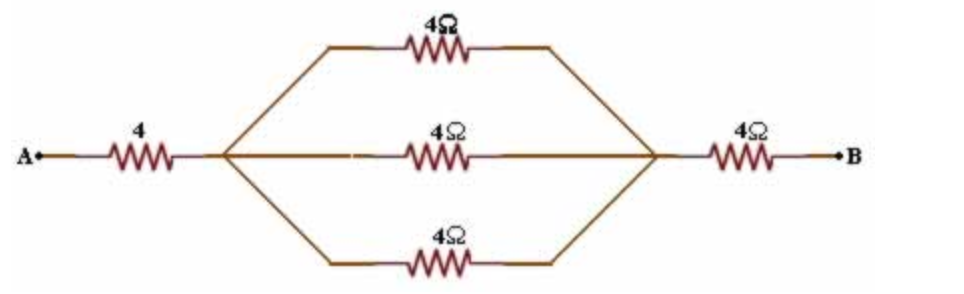
\includegraphics[width=0.8\linewidth]{Figuras/Ch15/ex02.PNG}}
}

\frame{
	\frametitle{Associação mista}
	\begin{block}{Exemplo \#03}
		Entre os pontos $A$ e $B$ do circuito abaixo é aplicada uma ddp de \SI{60}{\volt}.

		(a) Determine a intensidade de corrente no resistor de $\SI{10}{\ohm}$.

		(b) Qual é a ddp entre os extremos do resistor de $\SI{6}{\ohm}$?
	\end{block}

	\bigskip
	\centering
	\setmyunit{2cm}
	
	\begin{circuitikz}
		\draw (0,0) node[left] {$ A $} to[R=6<\ohm>,o-] ++(1.5,0)
		to[R=2<\ohm>] ++(1.5,0)
		to[R=3<\ohm>] ++(0,-1)
		to[R=5<\ohm>] ++(-1.5,0)
		to[R=4<\ohm>,-o] ++(-1.5,0) node[left] {$ B $}
		(1.5,0) to[R=10<\ohm>,*-*] ++(0,-1);
	\end{circuitikz}
%	\centerline{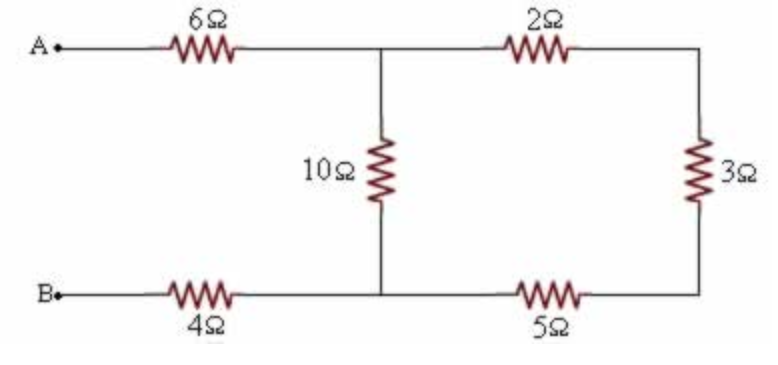
\includegraphics[width=0.8\linewidth]{Figuras/Ch15/ex03.PNG}}
}

\frame{
	\frametitle{Associação mista}
	\begin{block}{Exemplo \#04}
		Determine a resistência equivalente do seguinte circuito:
	\end{block}

	\centering
	\setmyunit{2cm}
	
	\ctikzset{resistors/scale=0.8}
	\begin{circuitikz}
		\draw (0,0) node[left] {$ A $} to[R=2.5<\ohm>,o-*] ++(1,0) -- ++(0,0.25)
		to[R=60<\ohm>] ++(1,0) -- ++(0,-0.25)
		++(-1,0) -- ++(0,-0.25) to[R=20<\ohm>] ++(1,0)
		to[short,-*] ++(0,0.25) -- ++(0.5,0)
		to[R=63<\ohm>,*-*] ++(0,-1.5)
		++(0,1.5) -- ++(0.5,0) -- ++(0,0.5)
		to[R=10<\ohm>] ++(1,0) -- ++(0,-1)
		to[R,a_=5<\ohm>] ++(-1,0) -- ++(0,0.5)
		to[R=10<\ohm>,*-*] ++(1,0)
		to[R=20.5<\ohm>] ++(1,0) -- ++(0,-1.5);
		
		\draw (0,-1.5) node[left] {$ B $} to[R=40<\ohm>,o-*] ++(1,0) -- ++(0,0.25)
		to[R=15<\ohm>] ++(1,0) -- ++(0,-0.25)
		++(-1,0) -- ++(0,-0.25) to[R=60<\ohm>] ++(1,0)
		to[short,-*] ++(0,0.25) -- ++(1,0) -- ++(0,0.5)
		to[R=30<\ohm>] ++(1,0) -- ++(0,-1)
		to[R,a_=30<\ohm>] ++(-1,0) -- ++(0,0.5)
		to[R=30<\ohm>,*-*] ++(1,0)
		to[R=30<\ohm>] ++(1,0);
	\end{circuitikz}
	
%	\centerline{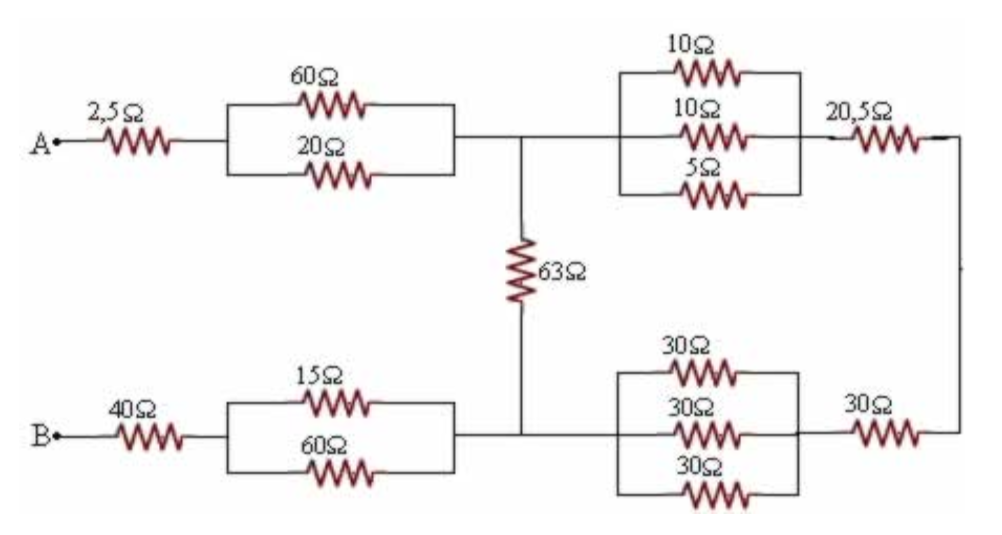
\includegraphics[width=0.9\linewidth]{Figuras/Ch15/ex04.PNG}}
}

\section*{Exercícios}

\frame{
	\frametitle{Exercícios}
	\begin{block}{}
		01. (UNISA-SP) Cinco resistores de \SI{200}{\ohm} cada são ligados, formando um quadrado com uma diagonal. Qual a resistência equivalente entre dois vértices, não adjacentes, ligados por um resistor?

		\vspace{0,5cm}

		02. (MACKENZIE-SP) No trecho de circuito representado a seguir, a potência dissipada pelo resistor de \SI{40}{\ohm} é \SI{10}{\watt}. Determine a intensidade de corrente elétrica que passa pelo resistor de \SI{2}{\ohm}.
	\end{block}

	\centering
	\setmyunit{2cm}
	
	\begin{circuitikz}
		\draw (0,0) to[R=2<\ohm>,o-] ++(1,0) -- ++(1,0) 
		to[R=40<\ohm>] ++(0,-1) -- ++(-1,0) ++(0,1) 
		to[R=10<\ohm>] ++(0,-1) to[short,-o] ++(-1,0);
		
		\draw[decorate,decoration={brace,amplitude=10pt,mirror,raise=4pt}] (0,0) -- node[left=15pt] {$ U $} (0,-1);
	\end{circuitikz}
%	\centerline{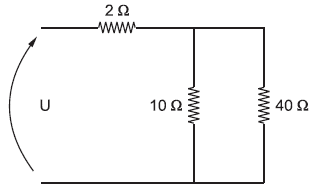
\includegraphics[width=0.5\linewidth]{Figuras/Ch15/exercicio.png}}
}

\section*{Referências}

\frame{
	\frametitle{Referências e Exercícios Complementares}
	\begin{itemize}
		\item Física, Ciência e Tecnologia – Vol 3. PENTEADO, Paulo César M; TORRES, Carlos Magno A. Ed. Moderna (2006)
	\end{itemize}
	%\centering{\alert{Página 36 - \textbf{1.6.1 até 1.6.5, 1.6.17 até 1.6.19}}} \\
	\centering{\alert{Lista de exercícios 15}}
}